%%%%%%%%%%%%%%%%%%%%%%%%%%%%%%%%%%%%%%%%%
% Short Sectioned Assignment LaTeX Template Version 1.0 (5/5/12)
% This template has been downloaded from: http://www.LaTeXTemplates.com
% Original author:  Frits Wenneker (http://www.howtotex.com)
% License: CC BY-NC-SA 3.0 (http://creativecommons.org/licenses/by-nc-sa/3.0/)
%%%%%%%%%%%%%%%%%%%%%%%%%%%%%%%%%%%%%%%%%

%----------------------------------------------------------------------------------------
%	PACKAGES AND OTHER DOCUMENT CONFIGURATIONS
%----------------------------------------------------------------------------------------

\documentclass[paper=a4, fontsize=11pt]{scrartcl} % A4 paper and 11pt font size

% ---- Entrada y salida de texto -----

\usepackage[T1]{fontenc} % Use 8-bit encoding that has 256 glyphs
\usepackage[utf8]{inputenc}
%\usepackage{fourier} % Use the Adobe Utopia font for the document - comment this line to return to the LaTeX default

% ---- Idioma --------

\usepackage[spanish, es-tabla]{babel} % Selecciona el español para palabras introducidas automáticamente, p.ej. "septiembre" en la fecha y especifica que se use la palabra Tabla en vez de Cuadro

% ---- Otros paquetes ----

\usepackage{url} % ,href} %para incluir URLs e hipervínculos dentro del texto (aunque hay que instalar href)
\usepackage{amsmath,amsfonts,amsthm} % Math packages
%\usepackage{graphics,graphicx, floatrow} %para incluir imágenes y notas en las imágenes
\usepackage{graphics,graphicx, float} %para incluir imágenes y colocarlas

% Para hacer tablas comlejas
%\usepackage{multirow}
%\usepackage{threeparttable}

%\usepackage{sectsty} % Allows customizing section commands
%\allsectionsfont{\centering \normalfont\scshape} % Make all sections centered, the default font and small caps

\usepackage{fancyhdr} % Custom headers and footers
\pagestyle{fancyplain} % Makes all pages in the document conform to the custom headers and footers
\usepackage{eurosym} % Para poder añadir el símbolo del euro
\fancyhead{} % No page header - if you want one, create it in the same way as the footers below
\fancyfoot[L]{} % Empty left footer
\fancyfoot[C]{} % Empty center footer
\fancyfoot[R]{\thepage} % Page numbering for right footer
\renewcommand{\headrulewidth}{0pt} % Remove header underlines
\renewcommand{\footrulewidth}{0pt} % Remove footer underlines
\setlength{\headheight}{13.6pt} % Customize the height of the header

\numberwithin{equation}{section} % Number equations within sections (i.e. 1.1, 1.2, 2.1, 2.2 instead of 1, 2, 3, 4)
%\numberwithin{figure}{section} % Number figures within sections (i.e. 1.1, 1.2, 2.1, 2.2 instead of 1, 2, 3, 4)
%\numberwithin{table}{section} % Number tables within sections (i.e. 1.1, 1.2, 2.1, 2.2 instead of 1, 2, 3, 4)

\setlength\parindent{0pt} % Removes all indentation from paragraphs - comment this line for an assignment with lots of text

\newcommand{\horrule}[1]{\rule{\linewidth}{#1}} % Create horizontal rule command with 1 argument of height

% Margins
\usepackage[margin=1.25in]{geometry}

% Begin section numbering at 0
\setcounter{section}{-1} 

% Hyperlinks
\usepackage{hyperref, xcolor}
\hypersetup{
  % hidelinks = true,   % Oculta todos los enlaces.
  colorlinks = true,   % Muestra todos los enlaces, sin bordes alrededor.
  linkcolor={black},     % Color de enlaces genéricos
  citecolor={black},   % Color de enlaces de referencias
  urlcolor={magenta}     % Color de enlaces de URL
}
  % Configuración del documento

%----------------------------------------------------------------------------------------
%	TÍTULO Y DATOS DE LOS ALUMNOS
%----------------------------------------------------------------------------------------

\title{	
	\normalfont \normalsize 
	\textsc{\textbf{Fundamentos de Redes (2017-2018)} \\ Doble Grado en Ingeniería Informática y Matemáticas \\ Universidad de Granada} \\ [25pt] 
	\horrule{0.5pt} \\[0.4cm]
	\huge Definición e implementación de un \\ protocolo de aplicación \\ 
	\horrule{2pt} \\[0.5cm] 
}

\author{Simón López Vico \\ Ana María Peña Arnedo \\ Alberto Jesús Durán López} 
\date{\normalsize\today}

%----------------------------------------------------------------------------------------
% DOCUMENTOg
%----------------------------------------------------------------------------------------

\begin{document}
	\maketitle       % título
	\newpage 
	\tableofcontents % índice
	\newpage
	
	

	
	
\section{Introducción}
	
	
Esta práctica consiste en la implementación de un protocolo de aplicación que consta
de un servidor y dos clientes. El juego se basa en el famoso "Pilla-Pilla"   donde 
un jugador 'X' tendrá que alcanzar a otro 'Y'. Para ello, ambos se conectarán con un nombre de usuario correcto almacenado en el servidor. Por tanto, los movimientos que ambos hagan se enviarán a través del servidor hacia el otro cliente.
		
	
	
	
\section{Diagrama de estados del servidor}

\begin{figure}[h]
	\centering
	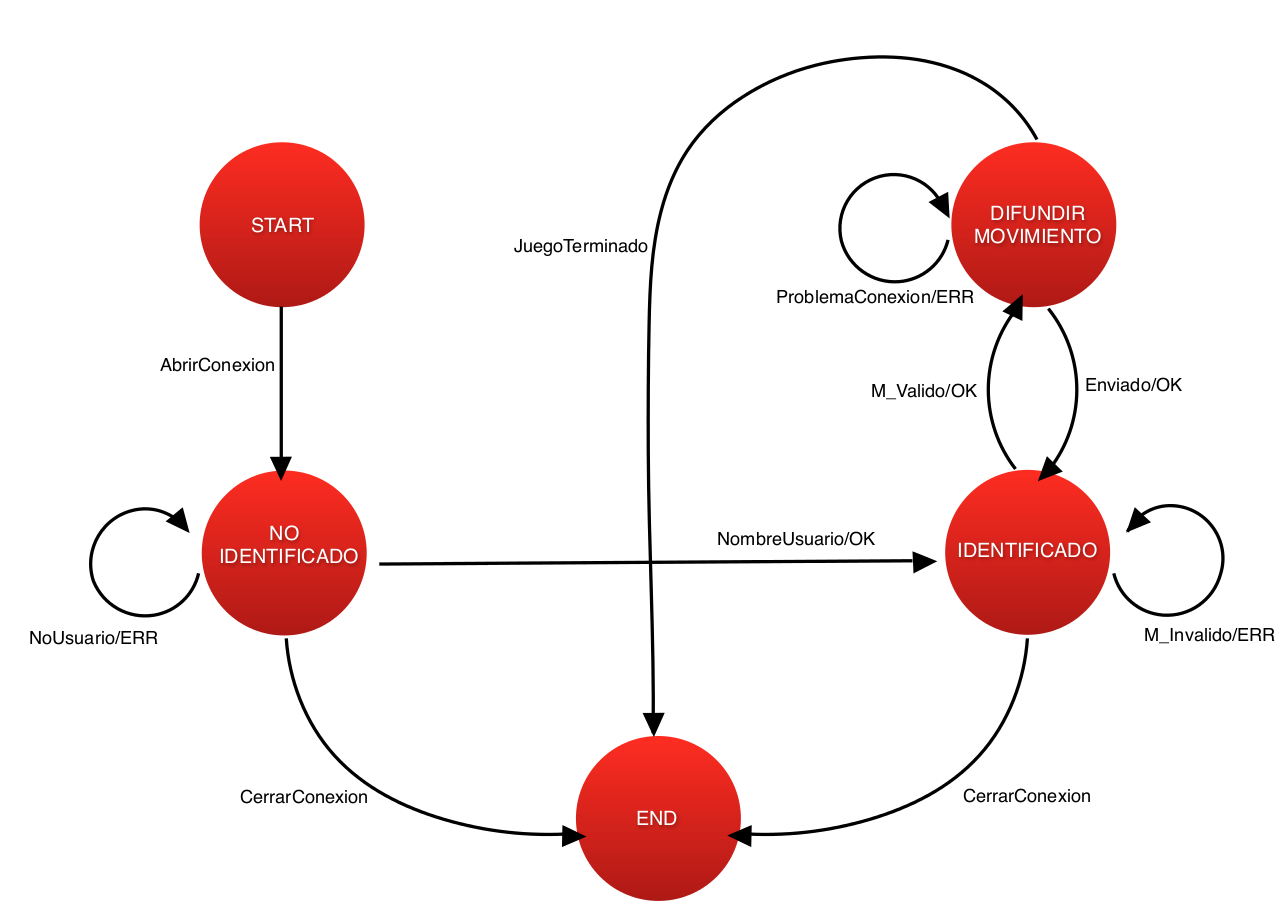
\includegraphics[width=.8\textwidth]{img/1}
	\caption{Diagrama de estados del servidor}
\end{figure}
	

Empezamos en el estado \textit{START}. El cliente abre la conexión hacia el servidor. Por tanto, pasará al estado \textit{IDENTIFICADO} si introduce un usuario correcto ó se quedará en el estado \textit{NO IDENTIFICADO} hasta que se autentifique correctamente. Una vez conectados ambos clientes, podrán realizar movimientos y pasar al estado \textit{DIFUNDIR MOVIMIENTO} un número indefinido de veces o pasar al estado \textit{END} si el juego se ha acabado. Cabe destacar que cada estado posee su propia comprobación de errores.
	












\newpage


\section{Tabla de estados del servidor}

\begin{figure}[h]
	\centering
	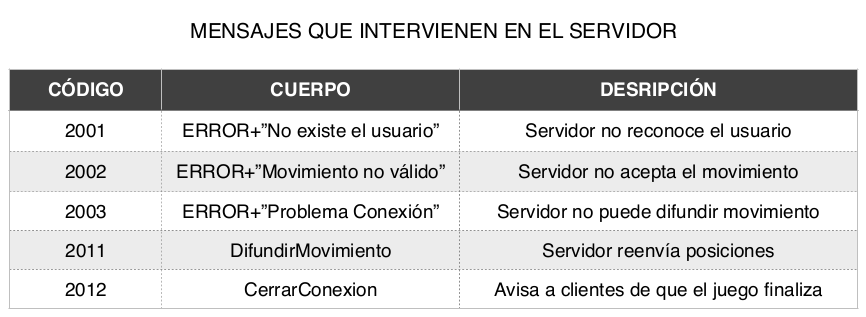
\includegraphics[width=.8\textwidth]{img/3}
	\caption{Mensajes que intervienen en el servidor}
\end{figure}


















\section{Tabla de estados del cliente}	

\begin{figure}[h]
	\centering
	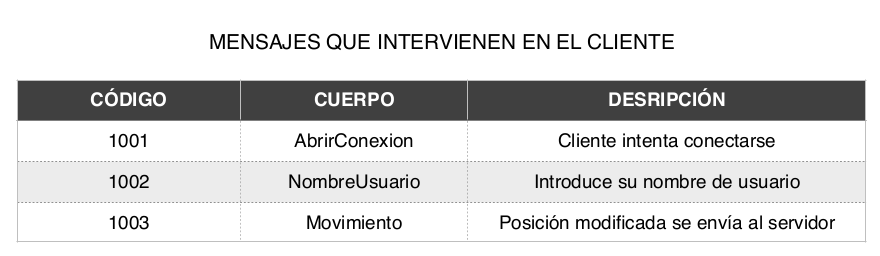
\includegraphics[width=.8\textwidth]{img/2}
	\caption{Mensajes que intervienen en el cliente}
\end{figure}













\end{document}